\documentclass[10pt,xcolor=dvipsnames,fontset=none,punct=CCT]{ctexbeamer}
\usetheme{Simple}
\usepackage{tikz,amsmath,amssymb}
\usepackage{unicode-math,mwe,array}
\usepackage{algorithm2e,multicol,siunitx}
\usepackage{ragged2e,minted,etoolbox,tabularray}
\usepackage{hyperref,xeCJKfntef,sidecap,pifont,booktabs,fontawesome5}
\hypersetup{
    colorlinks=true,
    linkcolor=,
}
\usetikzlibrary{tikzmark,arrows,scopes,shapes.geometric}
\tikzstyle{process} = [rectangle, minimum width=3cm, minimum height=1cm, text centered, draw=black, very thick, fill=gray!20]
\usepackage[citestyle=gb7714-2015,bibstyle=gb7714-2015]{biblatex}
\addbibresource{reference.bib}
\definecolor{mahiroLight}{RGB}{234,212,206}%选取小真寻头发的颜色作为最有特征的light的colbacktitle
\definecolor{mahiroCloth}{RGB}{228,243,248}%动画中小真寻人设图衣服的颜色作为colback
\definecolor{mahiroTrous}{RGB}{132,149,175}%动画中小真寻人设图裤子的颜色作为coltitle
\definecolor{mahiroSkins}{RGB}{255,228,212}%真寻酱的皮肤色,作为colframe

\definecolor{mahiroDark}{RGB}{234,212,206}%dark模式下真寻酱的发色
\definecolor{mahiroSchl}{RGB}{72,96,127}%人设图中真寻酱校服的颜色
\definecolor{mahiroLace}{RGB}{236,156,168}%真寻酱校服的花边颜色
% Commands for Highlighting text -- non tikz method
\newcommand{\highlight}[2]{\colorbox{#1!17}{#2}}
\apptocmd{\frame}{}{\justifying}{}
\linespread{1.3}
\setbeamertemplate{caption}[numbered]
\setminted{
  fontsize=\footnotesize,
  breaklines=true,
  breakanywhere=true
}

\newcolumntype{P}[1]{>{\centering\arraybackslash}p{#1}}

\PassOptionsToPackage{no-math}{fontspec}

\setCJKsansfont{Source Han Sans SC}[
  UprightFont=*-Regular,
  BoldFont=*-Bold
]
\setCJKmainfont{Source Han Sans SC}[
  UprightFont=*-Regular,
  BoldFont=*-Bold
]
% \setCJKmainfont{Source Han Serif SC}[
%   UprightFont=*-Regular,
%   BoldFont=*-Bold
% ]
\setCJKmonofont{FZFangSong-Z02}
\newCJKfontfamily\songti{Source Han Serif SC}[
  UprightFont=*-Regular,
  BoldFont=*-Bold
]
\newCJKfontfamily\heiti{Source Han Sans SC}[
  UprightFont=*-Regular,
  BoldFont=*-Bold
]
\newCJKfontfamily\fangsong{FZFangSong-Z02}
\newCJKfontfamily\kaishu{FZKai-Z03}
% \setmainfont{texgyrepagella}[
%   Extension      =.otf,
%   UprightFont    =*-regular,
%   BoldFont       =*-bold,
%   ItalicFont     =*-italic,
%   BoldItalicFont =*-bolditalic
% ]
\setmainfont{FiraSans}[
  Extension=.otf,
  UprightFont=*-Regular,
  BoldFont=*-Bold,
  ItalicFont=*-Italic
]
% \setsansfont{LinBiolinum}[
%   Extension=.otf,
%   UprightFont=*_R,
%   BoldFont=*_RB,
%   ItalicFont=*_RI
% ]
\setsansfont{FiraSans}[
  Extension=.otf,
  UprightFont=*-Regular,
  BoldFont=*-Bold,
  ItalicFont=*-Italic
]
\setmonofont{FiraMono}[
  Extension=.otf,
  UprightFont=*-Regular,
  BoldFont=*-Medium,
  ItalicFont=*-Oblique
]
% \setmathfont{texgyretermes-math.otf}[
%   Scale=MatchLowercase
% ]
% \setmathfont{latinmodern-math.otf}[
%   range=\int
% ]
\setmathfont{FiraMath-Regular.otf}
% \setmathfont{latinmodern-math.otf}
% \setmathrm{lmroman10-regular.otf}

\title[Maui Based Android Smartphone Development]{基于.NET 7 MAUI的PDR跨平台软件设计}
\subtitle{位置服务与实践答辩}

\author[LX Navi]{1组-崔宇璐\ 周天晨\ 陶安博}

\institute[WHU]
{
    Department of Navigation Engineering \\
    Wuhan University
}
\date{\today} 

% \mode<presentation>
% {
%   \setbeamercovered{transparent}
%   % or whatever (possibly just delete it)
% }

\AtBeginSubsection[]
{
  \begin{frame}<beamer>{Overview}
    \tableofcontents[currentsection,currentsubsection]
  \end{frame}
}

\begin{document}


\begin{frame}
  \titlepage
\end{frame}

\begin{frame}
  \frametitle{大纲}
  \tableofcontents
\end{frame}

\section{算法原理}
\subsection{行人航迹推算}

\begin{frame}
  \frametitle{Overview}
  航迹推算是依靠状态增量和姿态信息实现的无源导航手段.在二维平面上的航迹推算常常采用\textbf{行人航迹推算(Pedestrian Dead Reckoning, PDR)},其递推数学原理如下:
\begin{equation}\label{eq:PDR}
    \begin{cases}
        E_k=E_{k-1}+\hat{s}_{k-1,k}\cdot\sin\psi_{k-1}\\
        N_k=N_{k-1}+\hat{s}_{k-1,k}\cdot\cos\psi_{k-1}
    \end{cases}
\end{equation}
式中$(E_k,N_k)^T$是当前时刻平面位置,\ $(E_{k-1},N_{k-1})^T$是前一时刻平面位置,\ $\hat{s}_{k-1,k}$是从前一时刻迈向后一时刻的\textbf{步长},\ $\psi_{k-1}$是上一时刻\textbf{航向}角.
\end{frame}

\begin{frame}
  \frametitle{PDR流程}
  \begin{figure}
  \centering
  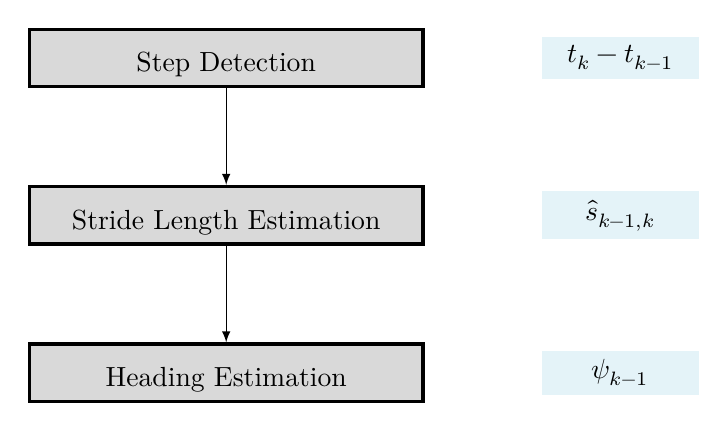
\begin{tikzpicture}
    {[every node/.style={draw, very thick, fill=gray!30, align=center, minimum width=5cm}]
    \node (SD) at (0,0) {步伐探测\\Step Detection};
    \node (SLE) at (0,-2) {步长估计\\Stride Length Estimation};
    \node (HE) at (0,-4) {航向估计\\Heading Estimation};
    }
    {[every node/.style={right=4cm, draw=white, fill=mahiroCloth, minimum width=2cm}]
    \node (SD-text) at (SD) {$t_{k}-t_{k-1}$};
    \node (SLE-text) at (SLE) {$\hat{s}_{k-1,k}$};
    \node (HE-text) at (HE) {$\psi_{k-1}$};
    }
    {[-latex]
      \draw (SD) -- (SLE);
      \draw (SLE) -- (HE);
    }
  \end{tikzpicture}
  \end{figure}
\end{frame}

\begin{frame}
  \frametitle{手机持平姿态下的步伐探测}
  \begin{itemize}
    \item 我们的实验在\CJKunderline{平坦地形}、\CJKunderline{手机持平}、\CJKunderline{步频稳定}的条件下进行
    \item 在这种实验条件下,加速度计测量值呈周期往复的正弦波形\cite{Bassett2016}
  \end{itemize}
  \begin{figure}[ht]
    \centering
    \includegraphics[width=0.6\linewidth]{figures/Accl.pdf}
  \end{figure}
\end{frame}

\begin{frame}
  \frametitle{基于峰值探测的步伐探测}
  \begin{itemize}
    \item 峰值探测(Peak Detection)利用行人连续行走的\CJKunderline{周期性}进行计数
    \item 然而,伪峰值(pseudo-peak)限制了峰值探测的精度
  \end{itemize}
  \begin{figure}[ht]
    \centering
    \includegraphics[width=0.6\linewidth]{figures/Accl.pdf}
  \end{figure}
\end{frame}

\begin{frame}
  \frametitle{滑动窗口平均}
  \begin{itemize}
    \item 可以采用滑窗滤波的方法来削弱多峰值的现象\cite{Zhang2017}
    \item 这种方法较为普遍,算法简单
    \item 缺点是会使数据丢失特性
  \end{itemize}
  \begin{columns}
  \column{0.65\linewidth}
  \begin{figure}[ht]
    \centering
    \includegraphics[width=0.85\linewidth]{figures/Smooth.pdf}
  \end{figure}
  \column{0.35\linewidth}
  \begin{gather}
    a(k)=\sqrt{a_x^2+a_y^2+a_z^2}\\
    \bar{a}(k)=\frac{1}{N}\sum_{i=k-N+1}^ka_c(i)
  \end{gather}
  \end{columns}
\end{frame}

\begin{frame}
  \frametitle{步伐探测}
  \begin{itemize}
    \item 设置加速度计阈值,以谷值为基准,若谷值小于阈值,则加入候选
    \item 设置时间阈值,若两探测信号之间的时间小于阈值,则不予探测成功
  \end{itemize}
  \begin{equation}
    \begin{cases}
      (a_k-a_{k-1})(a_{k+1}-a_k)<0,\\
      t_k-t_{k-1}>TH_t,\\
      a_k<TH_a
    \end{cases}\rightarrow\mathrm{is\ step}
  \end{equation}
\end{frame}

\begin{frame}
  \frametitle{步长估计}
  \begin{itemize}
    \item 对于同一个人,行走时的步长会有$\pm 40\%$的差异,且依赖于行走的速度
    \item 对于不同个体,步长依赖于腿长
    \item 因此设置常值步长会造成低精度
  \end{itemize}
  \begin{block}{步长估计经验模型模型\cite{Weinberg2002UsingTA}}
  \begin{columns}
  \column{0.6\linewidth}
    \[\mathrm{SL}\approx\sqrt[4]{a_\mathrm{peak}-a_\mathrm{valley}}\times K\]
    式中$a_\mathrm{peak}$为加速度计峰值,$a_\mathrm{valley}$为对应谷值,$K$为待确定的单位转换参数
  \column{0.3\linewidth}
  \begin{figure}
    \centering
    \includegraphics[width=\linewidth]{figures/foot.pdf}
  \end{figure}
  \end{columns}
  \end{block}
\end{frame}

\begin{frame}
  \frametitle{航向估计}
  移动设备的航向被定义为\CJKunderline{设备坐标系}和\CJKunderline{参考坐标系}之间的相对朝向关系\\
  如果选择磁强计数据来计算航向,流程如下:
\begin{figure}[ht]
    \centering
    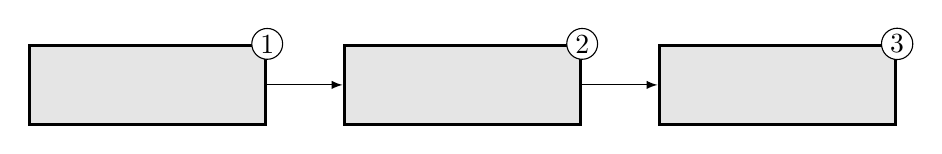
\begin{tikzpicture}
        \node[process] (A) at (0,0) {调平磁强计数据};
        \node[process] (B) at (4,0) {计算磁北航线};
        \node[process] (C) at (8,0) {计算真北航向};
        \node[draw,fill=white,circle,inner sep=1pt] at (A.north east) {1};
        \node[draw,fill=white,circle,inner sep=1pt] at (B.north east) {2};
        \node[draw,fill=white,circle,inner sep=1pt] at (C.north east) {3};
        \begin{scope}[-latex]
            \draw (A) -- (B);
            \draw (B) -- (C);
        \end{scope}
    \end{tikzpicture}
\end{figure}
\begin{enumerate}
    \item[\ding{172}] $\symbfit{m}^{\mathrm{n}_\ell}=\symbfit{C}_\mathrm{b}^{\mathrm{n}_\ell}\symbfit{m}^\mathrm{b}$,
    \item[\ding{173}] $\psi_{\mathrm{m}'}=-\mathrm{atan}_2(m_{\smash{y}}^{\mathrm{n}_\ell},m_{\smash{x}}^{\mathrm{n}_\ell})$,
    \item[\ding{174}] $\psi_\mathrm{m}=\psi_{\mathrm{m}'}+D$,式中$D$为磁偏角.
\end{enumerate}
可以通过国际地磁参考场(IGRF)模型获取磁偏角。
\end{frame}
\begin{frame}
  \frametitle{航向估计}
如果选择陀螺仪数据来计算航向,流程如下:
\begin{figure}[ht]
    \centering
    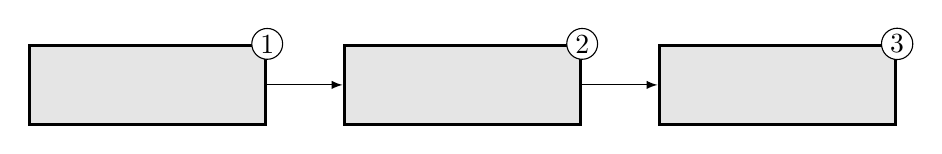
\begin{tikzpicture}
        \node[process] (A) at (0,0) {调平陀螺仪数据};
        \node[process] (B) at (4,0) {对时间求积分};
        \node[process] (C) at (8,0) {和上一时刻航向相加};
        \node[draw,fill=white,circle,inner sep=1pt] at (A.north east) {1};
        \node[draw,fill=white,circle,inner sep=1pt] at (B.north east) {2};
        \node[draw,fill=white,circle,inner sep=1pt] at (C.north east) {3};
    \begin{scope}[-latex]
        \draw (A) -- (B);
        \draw (B) -- (C);
    \end{scope}
    \end{tikzpicture}
\end{figure}
\begin{enumerate}
    \item[\ding{172}] 直接计算垂向角速度增量$\omega_D=[-\sin\theta,\sin r\cos\theta,\cos r\cos\theta]\symbfit{\omega}_\mathrm{ib}^\mathrm{b}$,
    \item[\ding{173}] $\Delta\psi=\int\omega_D\,\mathrm{d}t$,
    \item[\ding{174}] $\psi_k=\psi_{k-1}+\Delta\psi$.
\end{enumerate}
此处的陀螺仪输出视为与时间无关的常量,那么$\Delta\psi=\omega_D\Delta t$。
\end{frame}

\subsection{GCJ-02坐标转换}
\begin{frame}
  \frametitle{中国地图偏移问题}
  \begin{columns}[c]
    \column{.38\linewidth}
    \begin{figure}[ht]
      \centering
      \includegraphics[width=\columnwidth]{figures/shift.png}
    \end{figure}

    \column{.61\linewidth}
    \setlength{\parskip}{7pt plus 3pt minus 2pt}
    \begin{itemize}
    \item 中国GPS偏移问题由GCJ-20和WGS-84基准面不同导致。GPS定位采用的坐标系为WGS-84,投影至以GCJ-02坐标系为基准的街景地图后,会产生非常大(有时超过 \qty{500}{m} )的偏移。
    \item Google Maps选取GCJ-02坐标系作为街景图的参考系,而卫星影像图仍采用WGS-84,所以会导致如左图所示偏移问题。
    \end{itemize}
  \end{columns}
\end{frame}

\begin{frame}[allowframebreaks]
  \frametitle{WGS-84和GCJ-02坐标系转换}
  经纬度的改正值公式如下\cite{wandergis}:
  \begin{align*}
    \varphi' &=-100+2x+3y+0.2y^2+0.1xy+0.2\sqrt{|x|}\\
    &\ {}+\frac23\left\{[20\sin 6\pi x+20\sin 2\pi x]+\left[20\sin \pi y+40\sin\left(\frac{\pi y}{3}\right)\right]\right.\\
    &\left.\ {}+\left[160\sin\left(\frac{\pi y}{12}\right)+300\sin\left(\frac{\pi y}{30}\right)\right]\right\},\\
    \lambda' &=300+x+2y+0.1(x^2+xy)+0.1\sqrt{|x|}\\
    &\ {}+\frac23\left\{[20\sin 6\pi x+20\sin 2\pi x]+\left[20\sin \pi x+40\sin\left(\frac{\pi x}{3}\right)\right]\right.\\
    &\left.\ {}+\left[150\sin\left(\frac{\pi x}{12}\right)+300\sin\left(\frac{\pi x}{30}\right)\right]\right\}.
  \end{align*}
  其中
  \begin{equation*}
  \begin{cases}
      x=\varphi-105.0,\\
      y=\lambda- 35.0.
  \end{cases}
  \end{equation*}
  之后计算固定值 $(\varphi_\mathrm{fix},\lambda_\mathrm{fix})$:
  \begin{gather*}
  \varphi_\mathrm{fix}=\frac{180\varphi'}{\pi}\cdot\frac{W^3}{a(1-e^2)},\\
  \lambda_\mathrm{fix}=\frac{180\lambda'}{\pi}\cdot\frac{W\cos\left(\mathrm{D2R}(\varphi')\right)}{a},
  \end{gather*}
  式中 $W=\sqrt{1-e^2\sin(\varphi')}$,$a$ 为地球长半径,$e$ 为第一偏心率。
\end{frame}

\section{程序设计}
\begin{frame}{Overview}
  \tableofcontents[currentsection,currentsubsection]
\end{frame}

\subsection{.NET 7 MAUI框架}
\begin{frame}
  \frametitle{Overview}
  \begin{itemize}
    \item 移动端传感器接口:\href{https://learn.microsoft.com/zh-cn/dotnet/maui/platform-integration/device/sensors?view=net-maui-7.0\&tabs=android\#orientation}{访问设备传感器\ \faWindows} 并进行时间序列图绘制
    \item 算法程序设计
    \item Google Maps接口:\href{https://developers.google.com/maps/documentation/android-sdk/get-api-key?hl=zh-cn}{申请key\ \faGoogle} 和\href{https://learn.microsoft.com/zh-cn/dotnet/maui/user-interface/controls/map?view=net-maui-7.0}{数据映射\ \faWindows}
  \end{itemize}
  \begin{figure}[ht]
    \centering
    \includegraphics[width=\linewidth]{figures/pdr.pdf}
  \end{figure}
\end{frame}

\begin{frame}[fragile]
  \frametitle{.NET 7 MAUI框架}
  \begin{itemize}
    \item \textcolor{red}{程序特色所在}
    \item 是一个跨平台框架,使用 \mintinline{text}{C#} 和 \mintinline{text}{XAML} 创建移动和桌面应用
    \item 同一份代码可以在安卓、iOS、macOS和Windows平台运行
  \end{itemize}
  \begin{figure}
    \centering
    \includegraphics[width=0.5\linewidth]{figures/maui.pdf}
  \end{figure}
\end{frame}

\begin{frame}
  \frametitle{采取MAUI框架的理由}
  \begin{itemize}
    \item 微软详尽的学习文档、良好的社区氛围
    \item 强大的集成能力,实现对接口的统一调用
    \item 减少学习成本(\texttt{Kotlin}),便于分工合作
  \end{itemize}
  \begin{table}
    \centering
    \tabcolsep=3pt
    \begin{tabular}{P{.07\linewidth}P{.29\linewidth}P{.29\linewidth}P{.29\linewidth}}
      \toprule
      & MAUI & Compose & 原生框架 \\ \midrule
      语言 & \texttt{C\#}、\texttt{XAML} & \texttt{Kotlin} & \texttt{Java} \\
      平台 & \textsf{Cross-Platform} & \textsf{Android} & \textsf{Android} \\
      \vskip 0.05mm 特点 & 跨平台、一份代码库、高效 & 去\texttt{XML}、自动检测页面更改 & 方便调用Android原生API \\ \bottomrule
      \end{tabular}
  \end{table}
\end{frame}


\subsection{数据可视化}
\begin{frame}[fragile]
  软件实现的主要功能如下:
  \begin{itemize}
    \item 对三轴加速度计、陀螺仪、磁强计的数据进行实时监测
    \item 对传感器数据进行实时的时间序列图绘制,可实现数据保存和分享
    \item 可以获取定位,并告知用户经纬度
    \item 可以在Google Maps中展示PDR推算轨迹
  \end{itemize}
  实现的方法如下:
  \begin{itemize}
    \item 使用 \mintinline{csharp}{public void ToggleAccelerometer()} 方法对加计进行监听
    \item 利用第三方控件 \mintinline{csharp}{Syncfusion.Maui.Charts} 进行时间序列图展示
    \item \nointerlineskip\begin{minted}[bgcolor=gray!10]{csharp}
public static Task<Location?> GetLocationAsync (GeolocationRequest request, CancellationToken cancelToken);
    \end{minted}

    \nointerlineskip 参数 \mintinline{csharp}{request} 表示确定设备位置时要使用的条件,\mintinline{csharp}{cancelToken} 表示用于取消操作的令牌。
  \end{itemize}
\end{frame}

\begin{frame}
  \begin{columns}
  \column{0.7\linewidth}
  \begin{figure}[ht]
    \centering
    \includegraphics[height=0.95\textheight]{figures/界面1.jpg}
    \includegraphics[height=0.95\textheight]{figures/界面2.jpg}
  \end{figure}
  \column{0.3\linewidth}
  功能:
  \begin{itemize}
    \item 实时监测
    \item 实时绘制
    \item 数据清除
    \item 数据导出
  \end{itemize}
  \end{columns}
\end{frame}

\begin{frame}
  \begin{columns}
    \column{0.3\linewidth}
    功能:
    \begin{itemize}
      \item GPS定位结果
      \item PDR路线绘制
      \item 步长设置
      \item 视图切换
    \end{itemize}
    \column{0.7\linewidth}
    \begin{figure}[ht]
      \centering
      \includegraphics[height=0.95\textheight]{figures/界面3.jpg}
      \includegraphics[height=0.95\textheight]{figures/界面5.jpg}
    \end{figure}
    \end{columns}
\end{frame}

\subsection{主要代码}
\begin{frame}[fragile]
  \frametitle{PDR}
  \begin{itemize}
    \item 底层采用\texttt{C\#}语言编写
    \item 设计了 \mintinline{csharp}{class DeadReckoning},其中包含航迹推算算法
    \item 设计了 \mintinline{csharp}{class DeadReckoningMeasurement},用于储存观测值
  \end{itemize}
  \begin{block}{函数成员}
  \begin{minted}{csharp}
public class DeadReckoning
{
  public Vector2 GetCurrentCoord(DeadReckoningMeasurement measurement);
  public double GetSmoothedAccelerationData(int size, double acceleration);
  private bool StepDetect(double acceleration);
}
  \end{minted}
  \end{block}
\end{frame}

\begin{frame}{Google Maps API}
  \begin{table}[htb]
    \centering
    \begin{tblr}{
      colspec={X[c,m]X[c,m]X[c,m]X[c,m]X[c,m]X[c,m]},
      hline{1,Z}={1pt},
      hline{2,3},
      cell{1}{1}={r=2}{c},
      cell{1}{2}={r=2}{c},
      cell{1}{3}={r=2}{c},
      cell{1}{4}={r=2}{c},
      cell{1}{5}={c=2}{c}
    }
    地图名 & 范围 & 精度 & 偏移问题 & API 和 SDK & \\ 
    & & & & 申请 & 使用 \\
    Google Maps & 全球 & 最高 & 存在 & 不便 & 文档详尽、接口丰富 \\
    Bing Maps & 全球 & 次之 & 存在 & 不便 & 微软出品 \\
    高德地图 & 中国地区 & 略低 & 无偏移 & 方便 & 接口单一 \\
    \end{tblr}
  \end{table}
  以 Google Maps 和高德地图为例,在 Android SDK 方面,高德地图只提供了 Java 代码的旧框架示例代码,而 Google Maps 对新的 Jetpack Compose 框架和微软的 MAUI 框架都有良好的支持。
\end{frame}

\begin{frame}[fragile]{Google Maps 使用}
  \begin{block}{添加线段}
  \begin{minted}{csharp}
Map map = new Map();
// 实例化一个线段
Polyline polyline = new Polyline
{
    StrokeColor = Colors.Blue,
    StrokeWidth = 12,
    Geopath =
    {
        new Location(47.6381401, -122.1317367),
        new Location(47.6381473, -122.1350841)
    }
};
// 添加线段到地图
map.MapElements.Add(polyline);
  \end{minted}
  \end{block}
\end{frame}



\section{结果展示及精度分析}
\begin{frame}{Overview}
  \tableofcontents[currentsection,currentsubsection]
\end{frame}

\subsection{中间结果}
\begin{frame}
  \begin{columns}
    \column{0.5\linewidth}
    \begin{figure}
      \centering
      \includegraphics[width=\linewidth]{figures/resultAccl.pdf}
    \end{figure}
    \column{0.5\linewidth}
    \begin{figure}
      \centering
      \includegraphics[width=\linewidth]{figures/resultYaw.pdf}
    \end{figure}
  \end{columns}
  \begin{itemize}
    \item 呈现明显的周期性
    \item 初始航向不稳定,算法有待改进
    \item 计步器计数结果为$1264$步
  \end{itemize}
\end{frame}

\subsection{精度分析}
\begin{frame}
  \begin{figure}
    \centering
    \includegraphics[width=.7\linewidth]{figures/result.pdf}
  \end{figure}
  \begin{itemize}
    \item 第一圈(大约 \qty{400}{m} 后),闭合差为 \qty{14.73}{m}
    \item 随后闭合差减小,结合航向角图像来看,第一圈的闭合差大是因为初始航向角没有对准导致的
  \end{itemize}
\end{frame}

\section*{参考文献}
\begin{frame}
  \frametitle{参考文献}
  \printbibliography
\end{frame}

\end{document}